This section explains why each classical method gets the area wrong, and by how much. In short:
counting voxel faces measures a staircase instead of the real surface, so it is always too high;
marching cubes on a black-and-white volume can only build a few triangle directions, so it leaves a
small zig-zag that never goes away; and marching cubes on the greyscale volume is very good on flat
surfaces but slightly too small on curved ones (because the scan blurs the surface) and too large on
noisy ones. Knowing where each error comes from tells us what a correction model has to learn.

\subsection{Voxel-face counting}
Consider a planar piece of surface with unit normal $\mathbf n=(n_x,n_y,n_z)$. Its digital
(staircase) version is made of voxel faces normal to the three axes, and the total area of the faces
normal to axis $i$ equals the projection of the true area onto the plane perpendicular to that axis.
The face-count area per unit true area is therefore
\begin{equation}
  r(\mathbf n) = |n_x| + |n_y| + |n_z|, \qquad 1 \le r \le \sqrt3 .
\end{equation}
It equals 1 only for axis-aligned surfaces (Fig.~\ref{fig:facetheory}). For normals distributed
uniformly on the sphere each component is uniform on $[-1,1]$, so $\mathbb E|n_i| = 1/2$ and
$\mathbb E\,r = 3/2$. The face count of a randomly oriented smooth object thus overestimates its area by
50\%, and since $r$ does not depend on the voxel size, refining the grid does not help. On a clean sphere
at $128^3$ we measure $+50.03\%$.

\begin{figure}[t]
  \centering
  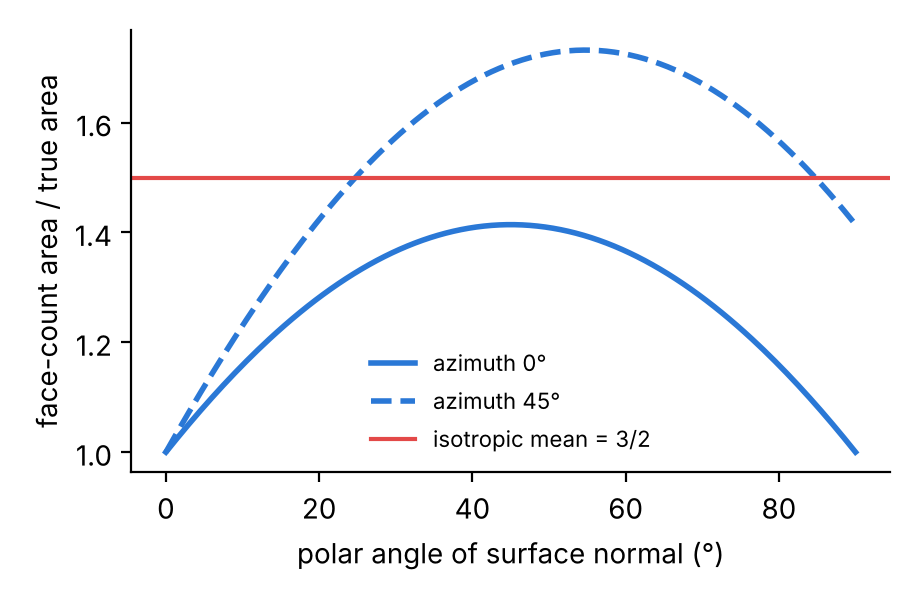
\includegraphics[width=0.52\linewidth]{face_count_theory.png}
  \caption{Face-count area per unit true area, $|n_x|+|n_y|+|n_z|$, for a plane whose normal makes the
  given polar angle with the $z$ axis, at azimuth 0° and 45°. The isotropic average is $3/2$.}
  \label{fig:facetheory}
\end{figure}

\subsection{Marching cubes on binary and greyscale volumes}
Marching cubes \citep{lorensen1987} places triangle vertices on the edges of each $2\times2\times2$
cell where the image crosses the iso-level. On a binary volume the crossing is always at the edge
midpoint, so only a finite set of triangle orientations can occur, and the mesh approximates a plane
of arbitrary orientation by a small-scale zig-zag whose excess area depends on the orientation but not
on the voxel size. Using smaller voxels makes the zig-zag finer but not flatter, so the area error does
not go to zero as the grid is refined \citep{kenmochi2000,svane2013}. On clean spheres we
measure $+7.3\%$ at $16^3$, rising to $+8.8\%$ at $128^3$.

On a greyscale volume the vertex position is interpolated from the partial-volume intensities, so
the mesh can follow the surface between voxel centres. For a flat surface the half-intensity level of
the blurred image lies exactly on the true surface. For a curved surface it does not: blurring spreads
the object's intensity outwards over a larger volume, so the half-intensity surface ends up slightly
inside the true one, and more so where the surface bends sharply. The result is an area that is a
little too small. For a sphere of radius $R$ voxels the expected error is about $-2\sigma^2/R^2$, where
$\sigma^2$ measures the total blur ($\sigma^2 \approx 0.44$ voxel$^2$ in our data). This predicts
$-0.56\%$ for a sphere on a $32^3$ grid, and we measure $-0.62\%$. The error shrinks quickly as objects
get larger, but extra smoothing (often used to remove noise) makes it about three times bigger. The
derivation and the full comparison are in Appendix~\ref{app:curvature}.

\subsection{Effect of noise}
Additive noise with standard deviation $\sigma_n$ has two effects on marching cubes. First, it perturbs
the iso-crossing positions near the surface. A randomly perturbed surface has more area than the
smooth one, since the area element $\sqrt{1+|\nabla\eta|^2}\ge1$ for any height perturbation $\eta$,
so this bias is always positive. Second, background voxels exceed the iso-level by chance with
probability $p = Q(0.5/\sigma_n)$, where $Q$ is the Gaussian tail function, and object voxels fall below
it with the same probability. Each such voxel becomes a tiny closed surface or cavity. For
$\sigma_n = 0.15$, $p = Q(3.33) \approx 4.3\times10^{-4}$, which predicts about 112 spurious components on
a $64^3$ grid and 14 on a $32^3$ grid. These specks can be counted with the Euler number of the
thresholded volume (roughly, the number of separate pieces and cavities minus the number of tunnels),
since each speck adds one to it. The measured Euler numbers at this noise level are indeed about 100 to
125 at $64^3$. For $\sigma_n = 0.05$, $p = Q(10)$ is negligible and only the surface roughening remains.
Gaussian smoothing removes most of this noise, but as explained above it also shrinks curved surfaces,
and it erases structures thinner than about $2\sigma_s$ entirely (we observe this for the thinnest tori
on the $32^3$ grid, where the smoothed volume never reaches the iso-level).

The upshot is that greyscale marching cubes has a negative, curvature-driven bias that grows at low
resolution, plus a positive, noise-driven bias that grows with $\sigma_n$ and with the number of
voxels. The two can partly cancel, which is why a single correction factor cannot fix both.

\subsection{Reference surface area}
Measuring the error of each method needs the true area of every shape. Spheres, cylinders, tori and
ellipsoids have exact formulas. Random blobs and superellipsoids do not, so their area is computed
numerically: the surface is covered with a very fine triangle mesh at two levels of detail (about
82,000 and 328,000 triangles), and the two results are combined to cancel the leading error term. The
remaining error is below 0.01\% for every shape, far smaller than the errors being measured. The
formulas are given in Appendix~\ref{app:reference}.

\subsection{Learning target}
All models predict
\begin{equation}
  y = \log\frac{A_\text{true}}{A_\text{MC}},
\end{equation}
where $A_\text{MC}$ is the greyscale marching-cubes area, and the final estimate is
$\hat A = A_\text{MC}\,e^{\hat y}$. The target is dimensionless, so it does not depend on the size of the
object, and it is invariant to rotations and translations of the object. This lets the training data
be augmented exactly with the 48 symmetries of the cube (axis permutations and reflections), which
permute voxels without interpolation and leave the true area unchanged.
